\begin{figure*}[t]
    \centering
    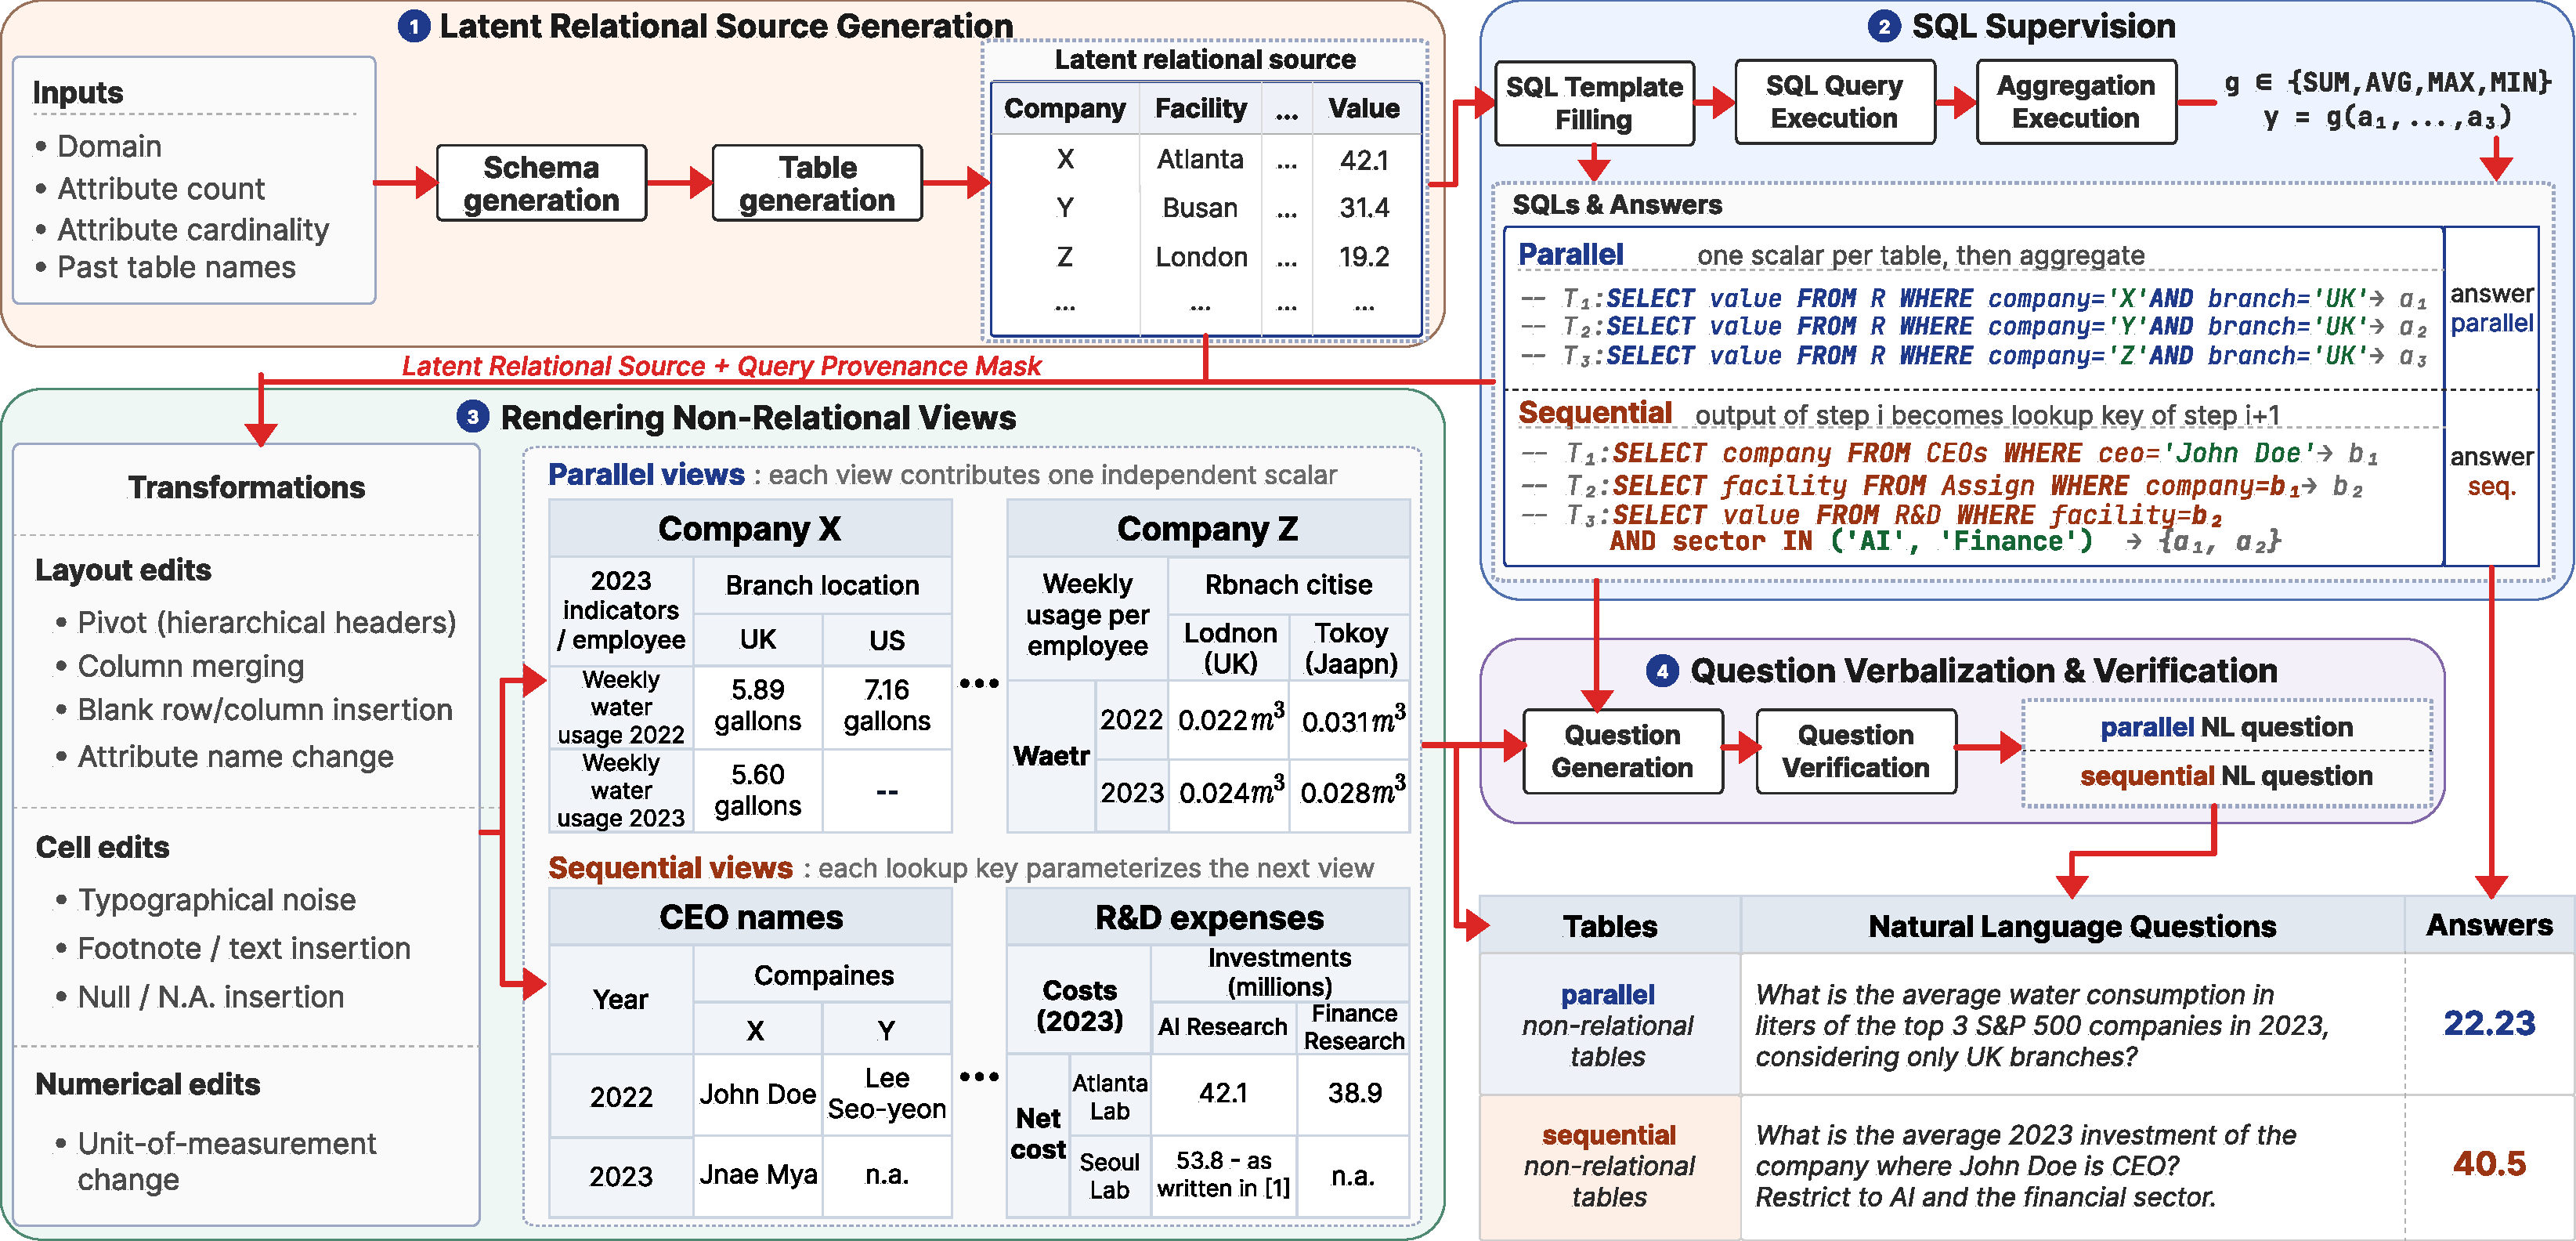
\includegraphics[width=\linewidth]{img/gradino.pdf}
    \caption{Overview of \name. A latent relational source provides SQL supervision and gold answers, while models are evaluated only on perturbed non-relational views.}
    \label{fig:pipeline}
    \vspace{-6pt}
\end{figure*}

\section{Related Work} 
\label{sec:rw}
\noindent{\bf Table QA benchmarks and robustness to tabular perturbations.}
Early Table QA benchmarks focused on relational tables, from single-table semantic parsing~\cite{1.4} to multi-table relational QA~\cite{1.6,1.19,1.20,1.30,pasupat2015,zhong2017seq2sql}. Subsequent studies showed that these systems remain brittle under schema, query, cell, and layout perturbations~\cite{2.4,2.5,2.6,2.8,2.9,2.10,szegedy2013,devlin2019bert}, as well as in realistic or domain-specific sources~\cite{2.7,5.7}. Non-relational Table QA benchmarks instead target semi-structured, hierarchical, or hybrid table-text inputs, where merged headers, layout cues, and irregular cell links make direct Text-to-SQL execution unsuitable~\cite{1.13,1.2,1.3,1.11,1.10,1.28,1.8,1.7,raffel2020,brown2020}. 
Beyond structural complexity, domain-specific benchmarks introduce specialized terminology and numerical reasoning challenges across areas such as finance, science, and environmental reporting~\cite{1.9,1.22,1.23,1.24,1.25,1.15,1.18,1.27,1.29}. Moreover, only a few benchmarks address non-relational multi-table reasoning: MultiHiertt~\cite{1.26} targets sequential reasoning over financial tables and text, whereas GRI-QA~\cite{1.16} requires parallel aggregation across environmental reports.
Although valuable, manually curated benchmarks are largely fixed in their domains, layouts, question distributions, perturbations, reasoning regimes, and number of tables. In contrast, \name is a configurable generation framework that provides control over parallel and sequential reasoning, table count, and structural, cell-level, layout, and numerical perturbations. Compared with existing benchmarks, this configurability enables systematic evaluation, model auditing, and domain-specific multi-table training at a scale that manual curation cannot support (\S\ref{sec:discussion}). 
\btitle{Automatic generation of tabular data.}
Synthetic Table QA and Text-to-SQL generation reduce annotation cost by sampling executable programs and verbalizing them into natural language, using SQL templates, query-diversification methods, or relational multi-hop constructions~\cite{9.2,9.5,9.6,9.7,9.8,5.5,5.8,zhong2017seq2sql,vaswani2017,raffel2020}. These methods usually start from existing relational databases, so they inherit fixed schemas, table counts, and question spaces. A separate line generates synthetic tables from examples or learned relational structure~\cite{5.1,5.9,5.10,5.2}, but targets tabular synthesis rather than QA. As summarized in \autoref{tab:related_work_comparison}, existing approaches generally address perturbation, table generation, or verifiable QA synthesis separately. 
In contrast, \name generates latent sources, non-relational views, executable answers, and multi-table questions from scratch, while allowing user guidance when higher domain realism is needed~\cite{5.12,brown2020} (§\ref{sec:semantic_constraints}).
\begin{comment}
Early Table QA benchmarks mainly targeted general-purpose QA over relational tables, including single-table semantic parsing~\cite{1.4} and multi-table relational QA~\cite{1.6,1.19,1.20,1.30}. These benchmarks supported the development of Text-to-SQL systems, but do not explicitly isolate cases where models fail. This limitation has motivated robustness studies on relational perturbations, such as schema synonyms~\cite{2.4}, distractor or replaced columns~\cite{2.5}, database, question, and SQL perturbations~\cite{2.6,2.8}, and tabular transposition and content reordering~\cite{2.9,2.10}. Other works show that relational QA remains difficult in realistic or domain-specific sources, including real user queries~\cite{2.7}, Kaggle and CTU databases~\cite{1.20}, and open data repositories~\cite{5.7}.
A different line of work focuses on non-relational tables, where merged headers, hierarchical layouts, and irregular semantic links between cells make direct Text-to-SQL execution unsuitable. General-purpose benchmarks include semi-structured tables~\cite{1.13,1.2,1.3,1.11}, hierarchical tables~\cite{1.10,1.28} and hybrid table-text QA~\cite{1.8,1.7}. Domain-specific benchmarks emphasize harder terminology and reasoning, especially in finance~\cite{1.9,1.22,1.23,1.24,1.25}, aviation~\cite{1.15}, education~\cite{1.18}, science~\cite{1.27,1.29}, and environmental reporting~\cite{1.16}. Multi-table non-relational benchmarks further increase complexity by requiring evidence aggregation across tables~\cite{1.26,1.16}.
These resources are valuable, but they are difficult to create for arbitrary domains, expensive to annotate at scale, and limited as training data or fine-grained auditing tools. \name addresses these limitations through a flexible generation pipeline. It reuses perturbations known to weaken models in relational settings, such as schema edits, distractors, and missing or noisy values~\cite{2.4,2.5,2.6,2.8}, but extends them to non-relational tables with additional structural and numerical perturbations, including pivots, layout changes, hierarchical headers, and unit conversions. Since users can control the topic, number of tables, and table size, \name reduces annotation costs, supports fast generation across domains, and enables stress-testing in larger multi-table settings, which previous benchmarks have shown to be particularly challenging~\cite{1.16,1.26}.
\btitle{Automatic generation of tabular data.}
The cost of manually annotating questions has motivated work on synthetic Table QA and Text-to-SQL data generation, typically by sampling executable programs and verbalizing them into natural language. Existing approaches use fixed SQL templates \cite{9.1,9.2,9.5}, improve the diversity and quality of generated queries \cite{9.6,9.7,9.8}, or construct questions requiring complex joins over relational sources \cite{5.5,5.8}. However, these methods usually start from existing relational databases. As a result, they inherit the structure and variability of the input tables, do not explicitly model tabular perturbations, and offer limited control over many-table settings and question types.
A related line of work generates synthetic tables that preserve the distribution or structure of input data. These methods rely on in-context examples \cite{5.1}, transformer-based relational generation \cite{5.9}, learned relational structure \cite{5.10}, or synthetic relational data models \cite{5.2}. Their goal, however, is primarily tabular synthesis rather than QA generation. Moreover, because generation is conditioned on existing tables, their flexibility across domains and reasoning settings remains limited.
In contrast, \name does not require any input table. This design enables end-to-end generation of tables with controllable structural and numerical properties, together with questions requiring reasoning over many tables, without human supervision. When higher realism is needed, users can also provide semi-automatic guidance to control the information used by \name during instance generation, following an approach similar to \citet{5.12} (see §\ref{sec:semantic_constraints}).
\end{comment} 
